\chapter{Notations tensorielles} \label{Ann:A}
L'objectif de cette annexe est de familiariser le lecteur avec les notations tensorielles.
Les résultats que nous démontrerons sont tout à fait classiques, et il convient de les considérer comme des exercices pour l'apprentissage des manipulations indicielles.
\section{Vecteurs et tenseurs}
\subsection{Notations indicielles}
Nous nous plaçons dans l'espace l'euclidien $E$ à trois dimensions.
Soit $\vec{e}_1$, $\vec{e}_2$, $\vec{e}_3$ une base orthonormée.
Un vecteur $\vec{V}$ est alors représenté par ses composantes $V_1$, $V_2$, $V_3$
\begin{equation}
    \vec{V} = V_1 \vec{e}_1 + V_2 \vec{e}_2 + V_3 \vec{e}_3 = V_i \vec{e}_i
    \label{eq:AnnA-001}
\end{equation}
en utilisant la convention de sommation: chaque fois que dans une expression un indice est répété, il convient de faire varier cet indice de 1 à 3 et de faire la somme.
Dans l'expression~\eqref{eq:AnnA-001}, l'indice $i$ e st un «~indice muet~»: on aurait aussi bien pu écrire $V_j \vec{e}_j$ ou $V_k \vec{e}_k$.

Soit $\mathbb{A}$ une application linéaire, alors dans la base $\vec{e}_1$, $\vec{e}_2$, $\vec{e}_3$,cette application est représentée par une matrice $3\times3$
\begin{equation}
    \mathbb{A} \text{ repr } 
    \begin{bmatrix}
        A_{11} & A_{12} & A_{13} \\    
        A_{21} & A_{22} & A_{23} \\    
        A_{31} & A_{32} & A_{33} 
    \end{bmatrix}
    \label{eq:AnnA-002}
\end{equation}
et, si $\vec{W} = \mathbb{A} \vec{V}$ les composantes de $\vec{W}$ sont données par
\begin{align*}
    W_1 &= A_{11} V_1 + A_{12} V_2 + A_{13} V_3\\
    W_2 &= A_{21} V_1 + A_{22} V_2 + A_{23} V_3\\
    W_3 &= A_{31} V_1 + A_{32} V_2 + A_{33} V_3
\end{align*}
que nous pouvons condenser en
\begin{equation}
    W_i = A_{ij} V_j
    \label{eq:AnnA-003}
\end{equation}
L'indice $j$ est un indice muet: on aurait aussi bien pu écrire $A_{ik} V_k$.
L' indice $i$ est un indice libre.
Dans une égalité, on doit avoir pour chaque terme les mêmes indices libres.

Nous introduisons les symboles de Kronecker
\begin{equation}
    \delta_{ij} = 
    \begin{cases} 
        1 & \text{ si } i = j\\
        0 & \text{ si } i \neq j
    \end{cases}
    \label{eq:AnnA-004}
\end{equation}
En particulier, l'application identité $\mathbb{I}$ est représentée par la matrice de composantes $\delta_{ij}$
\begin{displaymath}
    \mathbb{I} \text{ repr } 
    \begin{bmatrix}
        \delta_{11} & \delta_{12} & \delta_{13} \\
        \delta_{12} & \delta_{22} & \delta_{23} \\
        \delta_{31} & \delta_{32} & \delta_{33} 
    \end{bmatrix}
    =
    \begin{bmatrix}
        1 & 0 & 0 \\
        0 & 1 & 0 \\
        0 & 0 & 1
    \end{bmatrix}
\end{displaymath}
Si la base $\vec{e}_1$, $\vec{e}_2$, $\vec{e}_3$ est orthonormée, on a
\begin{equation}
    \vec{e}_i \cdot \vec{e}_j = \delta_{ij}
    \label{eq:AnnA-005}
\end{equation}
et le produit scalaire de deux vecteurs est
\begin{equation}
    \left\{
    \begin{aligned}
        \vec{V} \cdot \vec{W} &= V_i \vec{e}_i \cdot W_j \vec{e}_j = V_i W_j \vec{e}_i \cdot \vec{e}_j \\
        & = V_i W_j \delta_{ij}  =V_i W_i
    \end{aligned}
    \right.
    \label{eq:AnnA-006}
\end{equation}
De même, la composition de deux applications linéaires se traduît par le produit de leurs matrices représentatives, c'est à dire en notations indicielles
\begin{equation}
    \mathbb{C} = \mathbb{A} \circ \mathbb{B}, \qquad C_{ik} = A_{ij} B_{jk}
    \label{eq:AnnA-007}
\end{equation}
\subsection{Changement de repère}
Soit $\vec{e}_i$ une base orthonormée et $\vec{e}_i{}'$ une autre base orthonormée.
Soit $Q_{ij}$ la matrice de passage
\begin{align*}
    \vec{e}_1{}' &= Q_{11} \vec{e}_1 + Q_{12} \vec{e}_2 + Q_{13} \vec{e}_3 \\
    \vec{e}_2{}' &= Q_{21} \vec{e}_1 + Q_{22} \vec{e}_2 + Q_{23} \vec{e}_3 \\
    \vec{e}_3{}' &= Q_{31} \vec{e}_1 + Q_{32} \vec{e}_2 + Q_{33} \vec{e}_3 
\end{align*}
ou en notations indicielles
\begin{equation}
    \vec{e}_i{}' = Q_{ij} \vec{e}_j
    \label{eq:AnnA-008}
\end{equation}

Les deux bases étant orthonormées, on doit avoir
\begin{equation*}
    \delta_{ij} = \vec{e}_i{}' \cdot \vec{e}_j{}' = Q_{ik} Q_{jl} \vec{e}_k \cdot \vec{e}_l = Q_{ik} Q_{jk}
\end{equation*}
qui montre que la matrice inverse de $Q_{ij}$ est la matrice transposée
\begin{equation}
    Q_{ik}Q_{jk} = Q_{ki} Q_{kj} = \delta_{ij}
    \label{eq:AnnA-009}
\end{equation}
En particulier, on tire de \eqref{eq:AnnA-008} la relation inverse
\begin{equation}
    \vec{e}_j = Q_{kj} \vec{e}_k{}'
    \label{eq:AnnA-010}
\end{equation}
qui s'obtient par le calcul suivant: on multiplie \eqref{eq:AnnA-008} par $Q_{ik}$ et on utilise \eqref{eq:AnnA-009}
\begin{equation*}
    Q_{ik} \vec{e}_i{}' = Q_{ik} Q_{ij} \vec{e}_j = \delta_{kj} \vec{e}_j = \vec{e}_k
\end{equation*}
c'est à dire \eqref{eq:AnnA-010} à un changement d'indices près.
\subsection{Vecteurs}
Soit $\vec{V}$ un vecteur, $V_i$ ses composantes dans la base $\vec{e}_i$ et $V_i'$ celles dans la base $\vec{e}_i{}'$.
\begin{equation}
    \vec{V} = V_i \vec{e}_i = V_i' \vec{e}_i{}'
    \label{eq:AnnA-011}
\end{equation}
Pour obtenir 1es lois de transformation permettant de passer de nous utilisons \eqref{eq:AnnA-010}
\begin{displaymath}
    \vec{V} = V_i \vec{e}_i = V_i Q_{ki} \vec{e}_k{}'
\end{displaymath}
et par identification avec~\eqref{eq:AnnA-011}, il vient
\begin{equation}
    V_k' = Q_{ki} V_i, \qquad V_j =  Q_{ij} V_i'
    \label{eq:AnnA-012}
\end{equation}
formule de transformation des composantes d'un vecteur.

On appelle «~invariant~» une fonction des composantes d'un ou plusieurs vecteurs indépendante du repère choisi.
Par exemple, l'invariant produit scalaire est défini par
\begin{equation}
    \vec{V}\cdot \vec{W} = V_i W_i
    \label{eq:AnnA-013}
\end{equation}
C'est un invariant car, d'après \eqref{eq:AnnA-012} et \eqref{eq:AnnA-009},
\begin{displaymath}
    V_i' W_i' = Q_{ij} V_j Q_{ik} W_k = \delta_{jk} V_j W_k = V_j W_j
\end{displaymath}
\subsection{Applications linéaires}
Soit $\mathbb{A}$ une application linéaire de $E$ dans $E$. 
Dans la base $\vec{e}_i$, elle est représentée par une matrice $A_{ij}$ et dans la base $\vec{e}_i{}'$ par une autre matrice $A_{ij}'$.
Pour obtenir les lois de transformation, nous partons de \eqref{eq:AnnA-003} et de \eqref{eq:AnnA-012}
\begin{gather*}
    W_i = A_{ij} V_j \qquad W_i' = A_{ij}' V_j'\\
    W_i' = Q_{ik} W_k = Q_{ik} A_{kl} V_l = Q_{ik} A_{kl} Q_{jl} V_{j}'
\end{gather*}
et par identification il vient
\begin{equation}
    A_{ij}' = Q_{ik} Q_{jl} A_{kl}, \qquad A_{ij} = Q_{ki} Q_{lj} A_{kl}'
    \label{eq:AnnA-014}
\end{equation}
En particulier, on a vu que les symboles de Kronecker $\delta_{ij}$ étaient les composantes de la matrice associée à l'application identité. 
Par application de \eqref{eq:AnnA-014},
\begin{equation}
    \delta_{ij}' = Q_{ik} Q_{jl} \delta_{kl} = Q_{ik} Q_{jk} = \delta_{ij}
    \label{eq:AnnA-015}
\end{equation}
et l'application identité est représentée dans toute base par la même matrice.
\subsection{Formes bilinéaires}
Soit $A$ une forme bilinéaire sur $E$, c'est à dire une application bilinéaire $E\times E \rightarrow \mathbb{R}$.
Dans une base $\vec{e}_i$, elle est représentée par une matrice $A_{ij}$ telle que
\begin{equation}
    A \left( \vec{V}, \vec{W} \right) = A_{ij} V_i W_j
    \label{eq:AnnA-016}
\end{equation}
Pour obtenir la loi de transformation de $A_{ij}$ nous partons de \eqref{eq:AnnA-016} et de \eqref{eq:AnnA-012}
\begin{align}
    A\left( \vec{V}, \vec{W} \right) &= A_{ij} V_i W_j = A_{ij}' V_i'W_j'\\
    &= A_{ij} Q_{ki} V_k' Q_{lj} W_l' \nonumber
    \label{eq:AnnA-017}
\end{align}
d'où par identification
\begin{equation}
    A_{ij}' = Q_{ik} Q_{jl} A_{kl}, \qquad A_{ij} = Q_{ki} Q_{lj} A_{kl}'
    \label{eq:AnnA-018}
\end{equation}
c'est à dire la même loi de transformation que pour une application linéaire.
Ceci est évidemment dû au fait que nous n'envisageons que des repères orthonormés.
En particulier, la forme bilinéaire représentée dans toute base par les symboles de Kronecker est le produit scalaire.
\subsection{Tenseurs du second ordre}
Il résulte de ce qui précède que l'on peut identifier application linéaire et forme bilinéaire sur $E$.
Nous appellerons «~tenseur du 2nd ordre~» cette entité mathématique, généralisation de la notion de vecteur.
Algébriquement, on peut la définir en introduisant une opération bilinéaire «~produit tensoriel~», notée $\otimes$, et le tenseur $\mathbb{A}$ sera défini à partir de ses composantes $A_{ij}$ par
\begin{equation}
    \mathbb{A} = A_{ij} \vec{e}_i \otimes \vec{e}_j
    \label{eq:AnnA-019}
\end{equation}
formule qui généralise~\eqref{eq:AnnA-001}.
On obtient alors directement la loi de transformation~\eqref{eq:AnnA-014} ou \eqref{eq:AnnA-018} à partir de \eqref{eq:AnnA-008} ou \eqref{eq:AnnA-010}
\begin{gather*}
    \mathbb{A} = A_{ij} \vec{e}_i \otimes \vec{e}_j = A_{ij}' \vec{e}_i{}' \otimes \vec{e}_j{}'\\
    \begin{align*}
    \mathbb{A} = A_{ij} \vec{e}_i \otimes \vec{e}_j &= A_{ij} Q_{ki} \vec{e}_k{}' \otimes Q_{lj} \vec{e}_l{}'\\
    &= Q_{ki} Q_{lj} A_{ij} \vec{e}_k{}' \otimes \vec{e}_l{}'
    \end{align*}
\end{gather*}
d'où par identification
\begin{equation}
    A_{ij}' = Q_{ik} Q_{jl} A_{kl}, \qquad A_{ij} = Q_{ki} Q_{lj} A_{kl}'
    \label{eq:AnnA-020}
\end{equation}
et un tenseur du second ordre pourra représenter, suivant les circonstances, une application linéaire (exemple: le tenseur des contraintes) ou une forme bilinéaire (exemple: le tenseur des déformations).
Un tenseur sera dit \underline{symétrique} si
\begin{equation}
    A_{ij} = A_{ji}
    \label{eq:AnnA-021}
\end{equation}
\underline{antisymétrique} si
\begin{equation}
    A_{ij} = - A_{ji}
    \label{eq:AnnA-022}
\end{equation}
et \underline{isotrope} si
\begin{equation}
    A_{ij} = a \delta_{ij}
    \label{eq:AnnA-0123}
\end{equation}
Un tenseur quelconque peut toujours être décomposé en une partie symétrique $\mathbb{A}^S$ et une partie antisymétrique $\mathbb{A}^A$
\begin{equation}
    \begin{split}
        \mathbb{A} = \mathbb{A}^A + \mathbb{A}^S \quad A_{ij} = A_{ij}^A + A_{ij}^S \\
        A_{ij}^A = \frac{1}{2} \left( A_{ij} - A_{ji} \right), \quad A_{ij}^S = \frac{1}{2} \left( A_{ij} + A_{ji} \right)
    \end{split}
    \label{eq:AnnA-024}
\end{equation}
\subsection{Tenseurs n'ordre superieur}
Considérons, par exemple, une application linéaire de l'espace des tenseurs d'ordre deux dans lui-même (exemple: le tenseur d'élasticité).
Dans une base $\vec{e}_i$, il est représenté par une quantité $\Lambda_{ijkl}$ t à 4 indices
\begin{equation}
    \mathbb{A} = \lambda \left[ \mathbb{B} \right], \qquad A_{ij} = \Lambda_{ijkl} B_{kl}
    \label{eq:AnnA-025}
\end{equation}
La loi de transformation des $\Lambda_{ijkl}$ s'obtient directement à partir de~\eqref{eq:AnnA-018}
\begin{gather*}
    A_{ij} = \Lambda_{ijkl} B_{kl} \qquad A_{ij}' = \Lambda_{ijkl} B_{kl}'\\
    \begin{align*}
        A_{ij} &= Q_{im} Q_{jn} A_{mn} = Q_{im} Q_{jn} \Lambda_{mnkl} B_{kl}\\
        &= Q_{im} Q_{jn} Q_{pk} Q_{ql} \Lambda_{mnkl} B_{pq}'
    \end{align*}
\end{gather*}
d'où la loi de transformation
\begin{equation}
    \left\{
    \begin{aligned}
        \Lambda_{ijkl}' &= Q_{im} Q_{jn} Q_{kp} Q_{lp} \Lambda_{mnpq}\\
        \Lambda_{mnpq} &= Q_{im} Q_{jn} Q_{kp} Q_{lp} \Lambda_{ijkl}'
    \end{aligned}
    \right.
    \label{eq:AnnA-026}
\end{equation}
forme analogue à \eqref{eq:AnnA-020} ou \eqref{eq:AnnA-001}.
Nous introduisons donc le «~tenseur du 4-ème ordre~»
\begin{equation}
    \Lambda = \Lambda_{ijkl} \vec{e}_i \otimes \vec{e}_j \otimes \vec{e}_k \otimes \vec{e}_l
    \label{eq:AnnA-027}
\end{equation}
qui, suivant les circonstances, sera une application linéaire de l'espace des tenseurs du second ordre dans lui-même, une forme bilinéaire sur ce même espace, une forme quadrilinéaire sur l'espace des vecteurs, etc.
\subsection{Invariants}
On appelle «~invariant~» du tenseur du second ordre $\mathbb{A}$ une fonction des $A_{ij}$ indépendante du repère choisi.
Par exemple, 1es fonctions suivantes
\begin{equation}
    \left\{
    \begin{aligned}
        & \mathrm{tr} \mathbb{A} = A_{ii} \\
        & \mathrm{tr} \mathbb{A}^2 = A_{ij} A_{ji} , \qquad \mathrm{tr} \mathbb{A}^n = \cdots \\
        & \| \mathbb{A} \|^2 = A_{ij} A_{ij}
    \end{aligned}
    \right.
    \label{eq:AnnA-028}
\end{equation}
sont des invariants de $\mathbb{A}$.
En effet, on a par exemple
\begin{gather*}
    A_{ii}' = Q_{ik} Q_{il} A_{kl} = \delta_{kl} A_{kl} = A_{kk} \\
    \begin{align*}
        A_{ij}' A_{ij}' &= Q_{ik} Q_{jl} A_{kl} Q_{im} Q_{jn} A_{mn}\\
        &= \delta_{km} \delta_{ln} A_{kl} A_{mn} = A_{kl} A_{kl}, \quad \text{etc.}
    \end{align*}
\end{gather*}
On définit de la même manière les invariants de plusieurs tenseurs, ou d'un tenseur et de plusieurs vecteurs.
Par exemple, les quantités suivantes
\begin{equation}
    \left\{
    \begin{aligned}
        \mathrm{tr} \left( \mathbb{A} \mathbb{B} \mathbb{C} \right) &= A_{ij} B_{jk} C_{ki} \\
        \mathbb{A} : \mathbb{B} &= A_{ij} B_{ij} \\
        \vec{V}\cdot \mathbb{A} \vec{W} &= V_{i} A_{ij} W_j
    \end{aligned}
    \right.
    \label{eq:AnnA-029}
\end{equation}
sont des invariants.

En particulier, on remarque que $\mathbb{A}:\mathbb{B}$ définit un produit scalaire sur l'espace des tenseurs du second ordre.
Pour ce produit scalaire, l'espace des tenseurs symétriques est orthogonal à l'espace des tenseurs anti-symétriques.
En effet, si $\mathbb{A}$ est un tenseur symétrique et $\mathbb{\Omega}$ un tenseur anti-symétrique,
\begin{equation}
    A_{ij} A_{ji},\qquad \Omega_{ij} = -\Omega_{ji}
    \label{eq:AnnA-030}
\end{equation}
On a alors 
\begin{equation}
    \mathbb{A}:\mathbb{\Omega} = A_{ij} \Omega_{ij} = A_{ji} \Omega_{ji} = -A_{ij} \Omega_{ij} = 0
    \label{eq:AnnA-031}
\end{equation}
la première transformation résultant d'un échange des indices muets $i$ et $j$, la seconde de \eqref{eq:AnnA-030}.
De même, on peut décomposer un tenseur symétrique en partie sphérique et déviateur
\begin{equation}
    \mathbb{A} = \left( \frac{1}{3} \mathrm{tr} \mathbb{A} \right) \mathbb{I} + \mathbb{A}^D , \qquad A_{ii}^D = 0
    \label{eq:AnnA-032}
\end{equation}
et, à nouveau, c'est une décomposition en sous-espaces orthogonaux.

\section{Permutations et déterminants}
\subsection{Les symboles de permutation}
Nous introduisons les symboles de permutation
\begin{equation}
    \varepsilon_{ijk} = 
    \begin{cases}
        +1 & \text{ si } i, j, k \text{ permutation paire de } 1, 2, 3\\
        -1 & \text{ si } i, j, k \text{ permutation impaire de } 1, 2, 3\\
        0 & \text{ si deux indices sont répétés}
    \end{cases}
    \label{eq:AnnA-033}
\end{equation}
On peut relier ces symboles aux produits mixtes des vecteurs de base,
\begin{equation}
    \varepsilon_{ijk} = \left( \vec{e}_i, \vec{e}_j, \vec{e}_k \right)
    \label{eq:AnnA-034}
\end{equation}
On démontre alors sans difficulté (c'est une simple question de patience) les relations suivantes
\begin{equation}
    \begin{aligned}
        \varepsilon_{ijk} \varepsilon_{lmn} &= \det
            \begin{bmatrix}
                \delta_{il} & \delta_{im} & \delta_{in} \\
                \delta_{jl} & \delta_{jm} & \delta_{jn} \\
                \delta_{kl} & \delta_{km} & \delta_{kn}
            \end{bmatrix}\\
            \varepsilon_{ijk} \varepsilon_{imn} &= \delta_{jm} \delta_{kn} - \delta_{jn} \delta_{km} \\
            \varepsilon_{ijk} \varepsilon_{ijm} &=2 \delta_{km} \\
            \varepsilon_{ijk} \varepsilon_{ijk} &= 6 
    \end{aligned}
    \label{eq:AnnA-035}
\end{equation}
\subsection{Déterminant d'une matrice}
On peut démontrer que dans un changement de repère
\begin{equation}
    \varepsilon_{ijk}' = Q_{im} Q_{jn} Q_{kp} \varepsilon_{mnp} = \pm \varepsilon_{ijk}
    \label{eq:AnnA-036}
\end{equation}
suivant que le changement de base est direct ou non.
Si nous nous limitons aux repères orthonormés directs, alors
\begin{equation}
    \varepsilon_{ijk}' = \varepsilon_{ijk}
    \label{eq:AnnA-037}
\end{equation}
et les $\varepsilon_{ijk}$ sont les composantes d'un tenseur du 3ème ordre, qui représente, par exemple, la forme trilinéaire produit mixte
\begin{equation}
    \left( \vec{U}, \vec{V}, \vec{W} \right) = \varepsilon_{ijk} U_i V_j W_k
    \label{eq:AnnA-038}
\end{equation}
Les symboles de permutation permettent le calcul du déterminant d'une matrice par
\begin{equation}
    \varepsilon_{ijk} \det A = \varepsilon_{mnp} A_{im} A_{jn} A_{kp}
    \label{eq:AnnA-039}
\end{equation}
ou par \eqref{eq:AnnA-035}
\begin{equation}
    \det A = \frac{1}{6} \varepsilon_{ijk} \varepsilon_{mnp} A_{im} A_{jn} A_{kp}
    \label{eq:AnnA-040}
\end{equation}
En particulier, d'après \eqref{eq:AnnA-036}, $\det A$ est un invariant du tenseur du second ordre $\mathbb{A}$.
On peut également donner pour l'inverse d'une matrice (ou d'un tenseur) l'expression suivante
\begin{equation}
    \mathbb{B} = \mathbb{A}^{-1}, \quad B_{ji} = \frac{1}{2 \det \mathbb{A}} \varepsilon_{imn} \varepsilon_{jpq} A_{mp} A_{np}
    \label{eq:AnnA-041}
\end{equation}
En effet, on a, par \eqref{eq:AnnA-035} et \eqref{eq:AnnA-039},
\begin{align*}
    A_{ik} B_{kj} &= \frac{1}{2 \det \mathbb{A}} \varepsilon_{jmn} \varepsilon_{kpq} A_{ik} A_{mp} A_{nq} \\
    &= \frac{1}{2} \varepsilon_{jmn} \varepsilon_{imn} = \delta_{ij} \text{ c'est à dire } \mathbb{A} \mathbb{B} = \mathbb{I}
\end{align*}
\subsection{Polynôme caractéristique}
Les valeurs propres d'un tenseur du second ordre sont obtenues par résolution de l'équation caractéristique
\begin{equation}
    P\left( \lambda \right) = \det \left( \mathbb{A} - \lambda \mathbb{I} \right) = 0
    \label{eq:AnnA-042}
\end{equation}
soit, par développement de~\eqref{eq:AnnA-040}
\begin{displaymath}
    \frac{1}{6} \varepsilon_{ijk} \varepsilon_{mnp} \left( A_{im} -\lambda \delta_{im} \right) \left( A_{jn} - \lambda \delta_{jn} \right) \left( A_{kp} - \lambda \delta_{kp} \right) = 0
\end{displaymath}
\begin{equation}
    P\left( \lambda \right) = I_3 -\lambda I_2 + \lambda^{2} I_1 - \lambda^3
    \label{eq:AnnA-043}
\end{equation}
avec
\begin{equation}
    \left\{
    \begin{aligned}
        I_3 &= \frac{1}{6} \varepsilon_{ijk} \varepsilon_{mnp} A_{im} A_{jn} A_{kp} = \det \mathbb{A} \\
        I_2 &= \frac{1}{2} \left( A_{ii} A_{jj} - A_{ij} A_{ij} \right) = \frac{1}{2} \left[ \left( \operatorname{tr} \mathbb{A} \right)^2 - \operatorname{tr} \mathbb{A}^2 \right] \\
        I_1 &= A_{ii} = \operatorname{tr} \mathbb{A}
    \end{aligned}
    \right.
    \label{eq:AnnA-044}
\end{equation}
et $I_1$, $I_2$, $I_3$ sont appelés invariants fondamentaux du tenseur $\mathbb{A}$.
On peut montrer que tout invariant de $\mathbb{A}$ peut s'exprimer à partir de ces trois invariants fondamentaux.
Cela résulte, en particulier, de l'équation de Cayley-Hamilton
\begin{equation}
    P\left( \mathbb{A} \right) = I_3 \mathbb{I} - I_2 \mathbb{A} + I_1 \mathbb{A}^2 - \mathbb{A}^3
    \label{eq:AnnA-045}
\end{equation}
qui permet d'exprimer $\mathbb{A}$, et par récurrence $\mathbb{A}^4$, $\mathbb{A}^5$, etc. en fonction de $\mathbb{A}$ et $\mathbb{A}^2$.
\subsection{Adjoint d'un tenseur antisymétrique}
Soit il un tenseur antisymétrique.
Sa matrice représentative est
\begin{equation}
    \mathbb{\Omega} = 
    \begin{bmatrix}
        0 & \Omega_{12} & -\Omega_{31} \\
        -\Omega_{12} & 0 & \Omega_{23} \\
        \Omega_{31} & -\Omega_{23} & 0
    \end{bmatrix}
    \label{eq:AnnA-046}
\end{equation}
Nous pouvons lui associer le vecteur
\begin{equation}
    \vec{\omega} = 
    \begin{bmatrix}
        \omega_1 \\
        \omega_2 \\
        \omega_3
    \end{bmatrix} =
    \begin{bmatrix}
        \Omega_{23} \\
        \Omega_{31} \\
        \Omega_{12}
    \end{bmatrix}, \qquad
    \mathbb{\Omega} = 
    \begin{bmatrix}
        0 & \omega_3 &-\omega_2 \\
        -\omega_3 & 0 & \omega_1 \\
        \omega_2 & -\omega_1 & 0
    \end{bmatrix}
    \label{eq:AnnA-047}
\end{equation}
Le vecteur $\vec{\omega}$ est le vecteur adjoint du tenseur antisymétrique $\mathbb{\Omega}$.
Cette relation est exprimée par la relation
\begin{equation}
    \left\{
    \begin{aligned}
        \Omega_{ij} &= \varepsilon_{ijk} \omega_{k} \\
        \omega_i &= \frac{1}{2} \varepsilon_{ijk} \Omega_{jk}
    \end{aligned}
    \right.
    \label{eq:AnnA-048}
\end{equation}
En particulier, le vecteur $\vec{y} = \mathbb{\Omega} \vec{x}$ est donné par
\begin{equation}
    y_i = \Omega_{ij} x_j = \varepsilon_{ijk} \omega_k x_j
    \label{eq:AnnA-049}
\end{equation}
\section{Calcul vectoriel et analyse vectorielle}
\subsection{Calcul vectoriel}
On a vu que les notations indicielles permettaient d'exprimer simplement le produit scalaire par~\eqref{eq:AnnA-013} et le produit mixte par \eqref{eq:AnnA-038}.
Le produit vectoriel s'exprime aussi simplement par
\begin{equation}
    \vec{c} = \vec{a} \wedge \vec{b}, \qquad c_i = \varepsilon_{ijk} a_j b_k
    \label{eq:AnnA-050}
\end{equation}
comme on peut s'en convaincre par exemple en écrivant
\begin{displaymath}
    \vec{x}\cdot \left( \vec{a} \wedge \vec{b} \right) = \left( \vec{x}, \vec{a}, \vec{b} \right) = \varepsilon_{ijk} x_i a_j b_k
\end{displaymath}
ou bien par un calcul direct.

En particulier, si $\mathbb{\Omega}$ est un tenseur antisymétrique et $\vec{\omega}$ son vecteur adjoint, alors, si $\vec{y} = \mathbb{\Omega} \vec{x}$, on a par \eqref{eq:AnnA-048}
\begin{equation}
    \begin{aligned}
        y_i = \Omega_{ij} x_j = \varepsilon_{ijk} \omega_k x_j \\
        \mathbb{\Omega} \vec{x} = \vec{x} \wedge \vec{\omega}
    \end{aligned}
    \label{eq:AnnA-051}
\end{equation}
On peut également démontrer facilement les identités du calcul vectoriel, par exemple 
\begin{equation}
    \left( \vec{a} \wedge \vec{b} \right) \wedge \vec{c} = \left( \vec{a} \cdot \vec{c}  \right) \vec{b} - \left( \vec{b} \cdot \vec{c} \right) \vec{a}
    \label{eq:AnnA-052}
\end{equation}
\begin{equation}
    \left( \vec{a} \wedge \vec{b} \right) \cdot \left( \vec{c} \wedge \vec{d} \right) = \left( \vec{a} \cdot \vec{c} \right) \left( \vec{b} \cdot \vec{d} \right) - \left(  \vec{a} \cdot \vec{d} \right) \left( \vec{b} \cdot \vec{c} \right)
    \label{eq:AnnA-053}
\end{equation}
En effet, si $\vec{x} = \left( \vec{a} \wedge \vec{b} \right) \vec{c}$, on a d'après \eqref{eq:AnnA-050} et \eqref{eq:AnnA-035}
\begin{align*}
    x_i &= \varepsilon_{ijk} \varepsilon_{jmn} a_m b_n c_k = \varepsilon_{jki} \varepsilon_{jmn} a_m b_n c_k \\
    &= \left( \delta_{km} \delta_{in} - \delta_{kn} \delta_{im} \right) a_m b_n c_k \\
    &= a_k c_k b_i - b_k c_k a_i
\end{align*}
En guise d'exercice, on pourra démontrer de manière analogue \eqref{eq:AnnA-053}.
\subsection{Analyse vectorielle} \label{ssec:AnnA:3.2}
Nous considérons maintenant des fonctions à valeurs scalaires, vectorielles ou tensorielles, définies sur un ouvert $\Omega$.
Nous noterons d'une virgule la dérivée partielle par rapport à $x_i$
\begin{equation}
    {}_{,i} = \frac{\partial}{\partial x_i}
    \label{eq:AnnA-054}
\end{equation}
Par exemple, si $f$ est une fonction scalaire, nous définissons:
\begin{itemize}
    \item son gradient
        \begin{equation}
            \vec{\grad} f = f_{,i} \vec{e}_i \ \text{vecteur}
            \label{eq:AnnA-055}
        \end{equation}
    \item et son laplacien
        \begin{equation}
            \Delta f = f_{,ii} \ \text{scalaire}
            \label{eq:AnnA-056}
        \end{equation}
\end{itemize}

Si $\vec{v}$ est une fonction vectorielle, nous dêfinissons:
\begin{itemize}
    \item sa divergence
        \begin{equation}
            \dive \vec{v} = v_{i,i} \ \text{scalaire}
            \label{eq:AnnA-057}
        \end{equation}
    \item son rotationnel
        \begin{equation}
            \vec{\rot} \vec{v} = \varepsilon_{ijk} v_{k,j} \vec{e}_i \ \text{vecteur}
            \label{eq:AnnA-058}
        \end{equation}
    \item son gradient
        \begin{equation}
            \grad \vec{v} = v_{i,j} \vec{e}_i \otimes \vec{e}_j \ \text{tenseur}
            \label{eq:AnnA-059}
        \end{equation}
    \item son laplacien
        \begin{equation}
            \Delta \vec{v} = v_{i,jj} \vec{e}_i \ \text{vecteur}
            \label{eq:AnnA-060}
        \end{equation}
\end{itemize}
et l'on a, en particulier 
\begin{equation}
    \vec{\rot} \vec{\rot} \vec{v} = \vec{\grad} \dive \vec{v} \Delta \vec{v}
    \label{eq:AnnA-061}
\end{equation}

En effet, si $\vec{u} = \vec{\rot} \vec{\rot} \vec{v}$, on a, par \eqref{eq:AnnA-058} et \eqref{eq:AnnA-035},
\begin{align*}
    u_i &= \varepsilon_{ijk} \left( \varepsilon_{kmn} v_{n,m} \right)_{,j} \\
    &= \varepsilon_{kij} \varepsilon_{kmn} v_{n,mj} = v_{i,ij} - v_{i,jj}
\end{align*}
c'est à dire le second membre de \eqref{eq:AnnA-061}, par \eqref{eq:AnnA-055}, \eqref{eq:AnnA-057} et \eqref{eq:AnnA-060}.

Enfin,  si $\mathbb{A}$ est un tenseur, on définit sa divergence
\begin{equation}
    \dive \mathbb{A} = A_{ij,j} \vec{e}_i \ \text{vecteur}
    \label{eq:AnnA-062}
\end{equation}

On démontre alors facilement un certain nombre de relations utiles, par exemple,
\begin{align}
    \dive \left( f \vec{a} \right) & = f \dive \vec{a} + \vec{a} \cdot \grad f     \label{eq:AnnA-063}\\
    \dive \left( \vec{a} \wedge \vec{b} \right) &= \vec{b} \cdot \rot \vec{a} - \vec{a} \cdot \rot \vec{b}    \label{eq:AnnA-064}
\end{align}
et ainsi de suite.

\subsection{Transformations d'integrales}
\begin{wrapfigure}[4]{l}{.4\textwidth}
    \psset{unit=0.8cm}
    \centering
    \begin{pspicture}(0,0)(4.8,2.5)
        \psccurve(0.5,1.5)(4,2.3)(4.5,1.4)
        \rput(2.5,1.6){$\Omega$}
        \rput(0.2,2){$\partial \Omega$}
        \psline{->}(4,2.3)(4.8,2.6)
        \rput(4.3,2.8){$\vec{n}$}
    \end{pspicture}
\end{wrapfigure}
Soit $\Omega$ un domaine de l'espace, $\partial \Omega$ sa frontière,  et $\vec{n}$ sa  normale  extérieure.

On démontre  en  mathématiques  le théorème  suivant

\begin{thm}
Si $\phi$ est une fonction continue e·t à dérivée continue dans $\Omega$, et si $\partial \Omega$ admet un plan tangent continu par morceaux, alors on a
\begin{equation}
    \iiint_{\Omega} \phi_{,i} \ud v = \iint_{\partial \Omega} \phi n_i \ud S
    \label{eq:AnnA-065}
\end{equation}
\end{thm}
et toutes les formules de transformation d'intégrales utilisées dans ce cours peuvent se déduire de ce théorème.

\section{Coordonnées curvilignes}
Les formules du paragraphe~\ref{ssec:AnnA:3.2} et les formules que nous avons écrites dans ce cours sont valables en coordonnées cartésiennes.
En coordonnées curvilignes, il faut prendre quelques précautions, car les vecteurs de base changent.
Cela ne modifie en rien les relations entre tenseurs (par exemple, la loi de comportement), mais cela intervient chaque fois que l'on a des dérivations (par exemple, dans les équations d'équilibre ou dans la définition des déformations à partir des déplacements).
Nous allons donner un formulaire pour les coordonnées sphériques et cylindriques 

\subsection{Coordonnées cylindriques}
\begin{multicols}{2}
    \psfrag{x1}{$x_1$}
    \psfrag{x2}{$x_2$}
    \psfrag{x3}{$x_3$}
    \psfrag{er}{$\vec{e}_r$}
    \psfrag{et}{$\vec{e}_{\theta}$}
    \psfrag{ez}{$\vec{e}_z$}
    \psfrag{r}{$r$}
    \psfrag{t}{$\theta$}
    \psfrag{z}{$z$}
    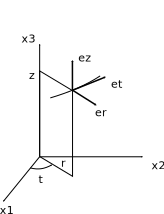
\includegraphics{../images/T1_AnnA-0002}
    \columnbreak

    Repère local: $\vec{e}_r,\ \vec{e}_{\theta},\ \vec{e}_{z}$
    \begin{displaymath}
        \vec{u} = 
        \begin{bmatrix}
            u_r \\
            u_{\theta} \\
            u_z
        \end{bmatrix}, \quad
        \mathbb{\sigma} = 
        \begin{bmatrix}
            \sigma_{rr} & \sigma_{r\theta} & \sigma_{rz} \\
            \sigma_{r\theta} & \sigma_{\theta\theta} & \sigma_{\theta z} \\
            \sigma_{rz} & \sigma_{\theta z} & \sigma_{zz} \\
        \end{bmatrix}
    \end{displaymath}
\end{multicols}

Gradient et Laplacien d'une fonction scalaire
\begin{align*}
    \grad f &= \frac{\partial f}{\partial r} \vec{e}_r + \frac{1}{r} \frac{\partial f}{\partial \theta} \vec{e}_{\theta} + \frac{\partial f}{\partial z} \vec{e}_z \\
    \Delta f &= \frac{1}{r} \frac{\partial}{\partial r} \left( r \frac{\partial f}{\partial r} \right) + \frac{1}{r^{2}}\frac{\partial^2 f}{\partial \theta^2} + \frac{\partial^2 f}{\partial z^2}
\end{align*}
Définition des déformations
\begin{align*}
    \varepsilon_{rr} &= \frac{\partial u_r}{\partial r} \quad \varepsilon_{\theta\theta} = \frac{1}{r} \frac{\partial u_{\theta}}{\theta} + \frac{u_r}{r} \quad \varepsilon_{zz} = \frac{\partial u_z}{\partial z} \\
    \varepsilon_{\theta z} &= \frac{1}{2} \left\{ \frac{1}{r} \frac{\partial u_z}{\theta} + \frac{\partial u_{\theta}}{\partial z} \right\} \quad \varepsilon_{rz} = \frac{1}{2} \left\{ \frac{\partial u_r}{\partial z} + \frac{\partial u_z}{\partial r} \right\} \\
    \varepsilon_{r\theta} &= \frac{1}{2} \left\{ \frac{\partial u_{\theta}}{\partial r} - \frac{u_{\theta}}{r} + \frac{1}{r} \frac{\partial u_r}{\partial \theta} \right\}
\end{align*}
Equations d'équilibre
\begin{align*}
    \frac{\partial \sigma_{rr}}{\partial r} + \frac{1}{r} \frac{\partial \sigma_{r\theta}}{\partial \theta} + \frac{\partial \sigma_{rz}}{\partial z} + \frac{\sigma_{rr} - \sigma_{\theta\theta}}{r} + f_r &=0\\
    \frac{\partial \sigma_{r\theta}}{\partial r} + \frac{1}{r} \frac{\partial \sigma_{\theta\theta}}{\partial \theta} + \frac{\partial \sigma_{\theta z}}{\partial z} + \frac{2\sigma_{r\theta}}{r} + f_{\theta} &=0\\
    \frac{\partial \sigma_{rz}}{\partial r} + \frac{1}{r} \frac{\partial \sigma_{\theta z}}{\partial \theta} + \frac{\partial \sigma_{zz}}{\partial z} + \frac{\sigma_{rz}}{r} + f_z &=0
\end{align*}

\subsection{Coordonnées sphériques}
\begin{multicols}{2}
    \psfrag{x1}{$x_1$}
    \psfrag{x2}{$x_2$}
    \psfrag{x3}{$x_3$}
    \psfrag{er}{$\vec{e}_r$}
    \psfrag{et}{$\vec{e}_{\theta}$}
    \psfrag{ep}{$\vec{e}_{\phi}$}
    \psfrag{r}{$r$}
    \psfrag{t}{$\theta$}
    \psfrag{p}{$\phi$}
    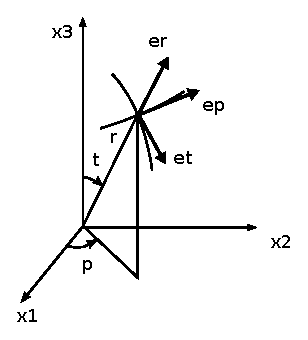
\includegraphics{../images/T1_AnnA-0003}
    \columnbreak

    Repère local: $\vec{e}_r,\ \vec{e}_{\theta},\ \vec{e}_{\phi}$
    \begin{displaymath}
        \vec{u} = 
        \begin{bmatrix}
            u_r \\
            u_{\theta} \\
            u_{\phi}
        \end{bmatrix}, \quad
        \mathbb{\sigma} = 
        \begin{bmatrix}
            \sigma_{rr} & \sigma_{r\theta} & \sigma_{r\phi} \\
            \sigma_{r\theta} & \sigma_{\theta\theta} & \sigma_{\theta\phi} \\
            \sigma_{r\phi} & \sigma_{\theta\phi} & \sigma_{\phi\phi} \\
        \end{bmatrix}
    \end{displaymath}
\end{multicols}

Gradient et Laplacien d'une fonction scalaire
\begin{align*}
    \grad f &= \frac{\partial f}{\partial r} \vec{e}_r + \frac{1}{r} \frac{\partial f}{\partial \theta} \vec{e}_{\theta} + \frac{1}{r\sin \theta} \frac{\partial f}{\partial \phi} \vec{e}_{\phi} \\
    \Delta f &= \frac{1}{r^2} \frac{\partial}{\partial r} \left( r^2 \frac{\partial f}{\partial r} \right) + \frac{1}{r\sin \theta} \frac{\partial}{\partial \theta}\left( \frac{\sin \theta}{r} \frac{\partial f}{\partial \theta} \right) + \frac{1}{r\sin \theta}\frac{\partial f}{\partial \phi} \left( \frac{1}{r\sin \theta} \frac{\partial f}{\partial \phi} \right)
\end{align*}
Définition des déformations
\begin{align*}
    \varepsilon_{rr} &= \frac{\partial u_r}{\partial r} \quad \varepsilon_{\theta\theta} = \frac{1}{r} \frac{\partial u_{\theta}}{\theta} + \frac{u_r}{r} \quad \varepsilon_{\phi\phi} = \frac{1}{r \sin \theta} \frac{\partial u_{\phi}}{\partial \phi} + \frac{u_{\theta}}{r}\cot \theta + \frac{u_r}{r} \\
    \varepsilon_{\theta \phi} &= \frac{1}{2r} \left\{ \frac{\partial u_{\phi}}{\theta} - u_{\phi} \cot \theta \right\} + \frac{1}{2r\sin \theta} \frac{\partial u_{\theta}}{\partial \phi} \\
    \varepsilon_{r\phi} &= \frac{1}{2} \left\{ \frac{1}{r \sin \theta} \frac{\partial u_r}{\partial \phi} + \frac{\partial u_\phi}{\partial r} - \frac{u_{\phi}}{r}\right\} \\
    \varepsilon_{r\theta} &= \frac{1}{2} \left\{ \frac{\partial u_{\theta}}{\partial r} - \frac{u_{\theta}}{r} + \frac{1}{r} \frac{\partial u_r}{\partial \theta} \right\}
\end{align*}
Equations d'équilibre
\begin{align*}
    \frac{\partial \sigma_{rr}}{\partial r} + \frac{1}{r} \frac{\partial \sigma_{r\theta}}{\partial \theta} + \frac{1}{r \sin \theta} \frac{\partial \sigma_{r\phi}}{\partial \phi} + \frac{2 \sigma_{rr} - \sigma_{\theta\theta} -\sigma_{\phi\phi} +\sigma_{r\theta} \cot \theta}{r} + f_r &=0\\
    \frac{\partial \sigma_{r\theta}}{\partial r} + \frac{1}{r} \frac{\partial \sigma_{\theta\theta}}{\partial \theta} + \frac{\partial \frac{1}{r \sin \theta} \sigma_{\theta \phi}}{\partial \phi} + \frac{1}{r} \left[ \left( \sigma_{\theta\theta} -\sigma_{\phi\phi} \right)\cot\theta +3\sigma_{r\theta} \right]+ f_{\theta} &=0\\
    \frac{\partial \sigma_{r\phi}}{\partial r} + \frac{1}{r} \frac{\partial \sigma_{\theta \phi}}{\partial \theta} + \frac{1}{r \sin \theta} \frac{\partial \sigma_{\phi\phi}}{\partial \phi} + \frac{1}{r}\left( 3\sigma_{r\phi} + 2 \sigma_{\theta\phi}\cot \theta \right) + f_\phi &=0
\end{align*}

